\documentclass[12pt, fleqn]{article}

\usepackage[left=0.75in, right=0.75in, bottom=0.75in, top=1.0in]{geometry}
\usepackage{amsmath}
\usepackage{amssymb}
\usepackage{amsthm}
\usepackage{mathtools}
\usepackage{hyperref}
\usepackage{ulem}
\usepackage{enumitem}
\usepackage{floatrow}
\usepackage{graphicx}
\usepackage[export]{adjustbox}
\usepackage{sectsty}
% \sectionfont{\centering}
\renewcommand*{\thesubsection}{\alph{subsection}.}

\usepackage[dvipsnames]{xcolor}
\usepackage[perpage]{footmisc}

\usepackage{fancyhdr}
\pagestyle{fancy}
\fancyhf{}
\lhead{190100044}
\rhead{CS 341 Assignment 3}
\renewcommand{\footrulewidth}{1.0pt}
\cfoot{Page \thepage}

\setlength{\parindent}{0em}

\title{CS 341 Assignment 3}
\author{Devansh Jain, 190100044}
\date{\today}

\begin{document}

% \pagenumbering{gobble}
\maketitle
\tableofcontents
\thispagestyle{empty}
\setcounter{page}{0}

\newpage
\section{5 Stage, without forwarding or hazard detection}

\subsubsection*{Code}
\begin{verbatim}
.text

main:
    addi s0 zero 5
    add s1 s0 zero
\end{verbatim}

\subsubsection*{Behaviour}
Expectation: At the end of the program, we expect registers \verb!s0! and \verb!s1! to have value 5. \\
Reality: At the end of the program, only register \verb!s0! has value 5. (\verb!s1! is default to 0)

\subsubsection*{Explanation}
The incorrect value is due to data hazard. \\
To be more specific, we face a \textbf{read-before-write (RAW) data hazard}. \\
\verb!addi s0 zero 5! writes to register \verb!s0! in WB stage during 4th cycle. \\
\verb!add s1 s0 zero! reads from register \verb!s0! in ID stage during 2nd cycle. \\
The value read here is not updated yet causing the incorrect computation.

\subsubsection*{Screenshots}
\begin{figure}[H]
  \centering
  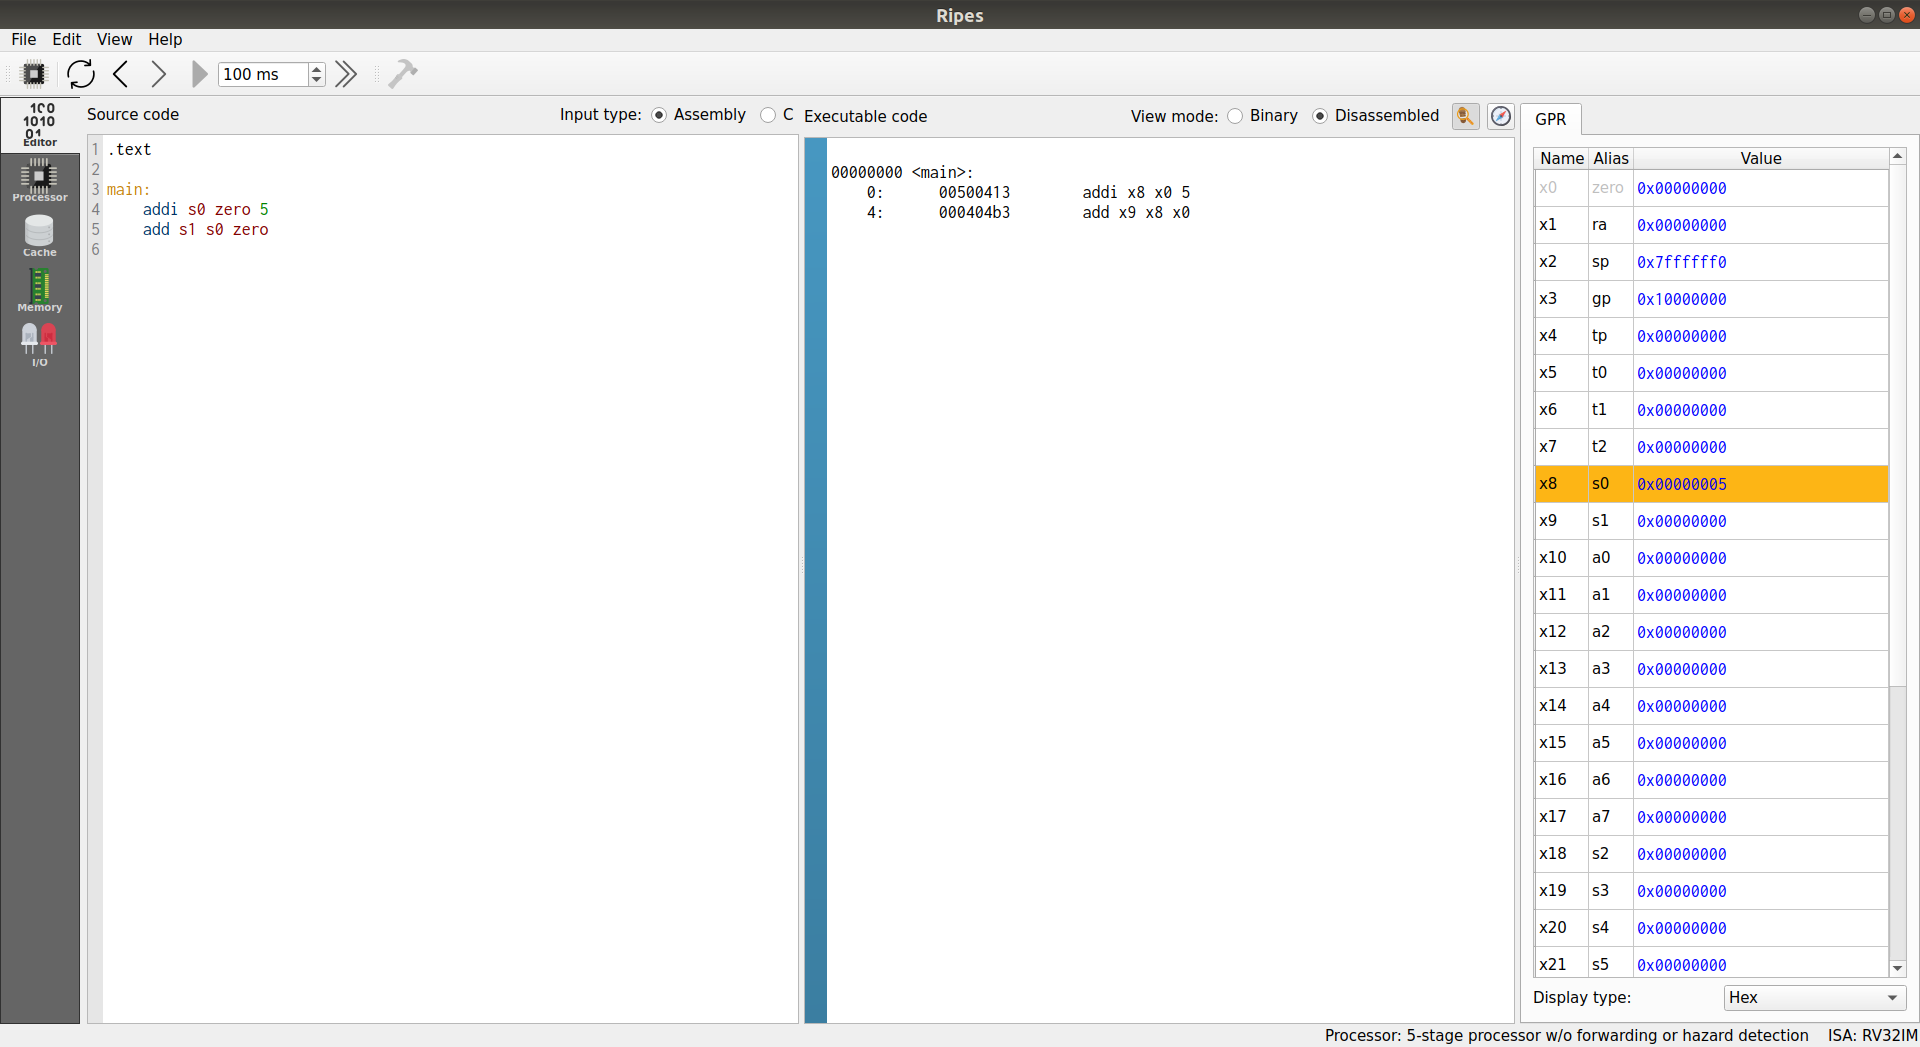
\includegraphics[scale=0.25]{Q1/nhnf_end_editor.png}
  \caption{Without hazard detection; Without forwarding;}
\end{figure}
\begin{figure}[H]
  \centering
  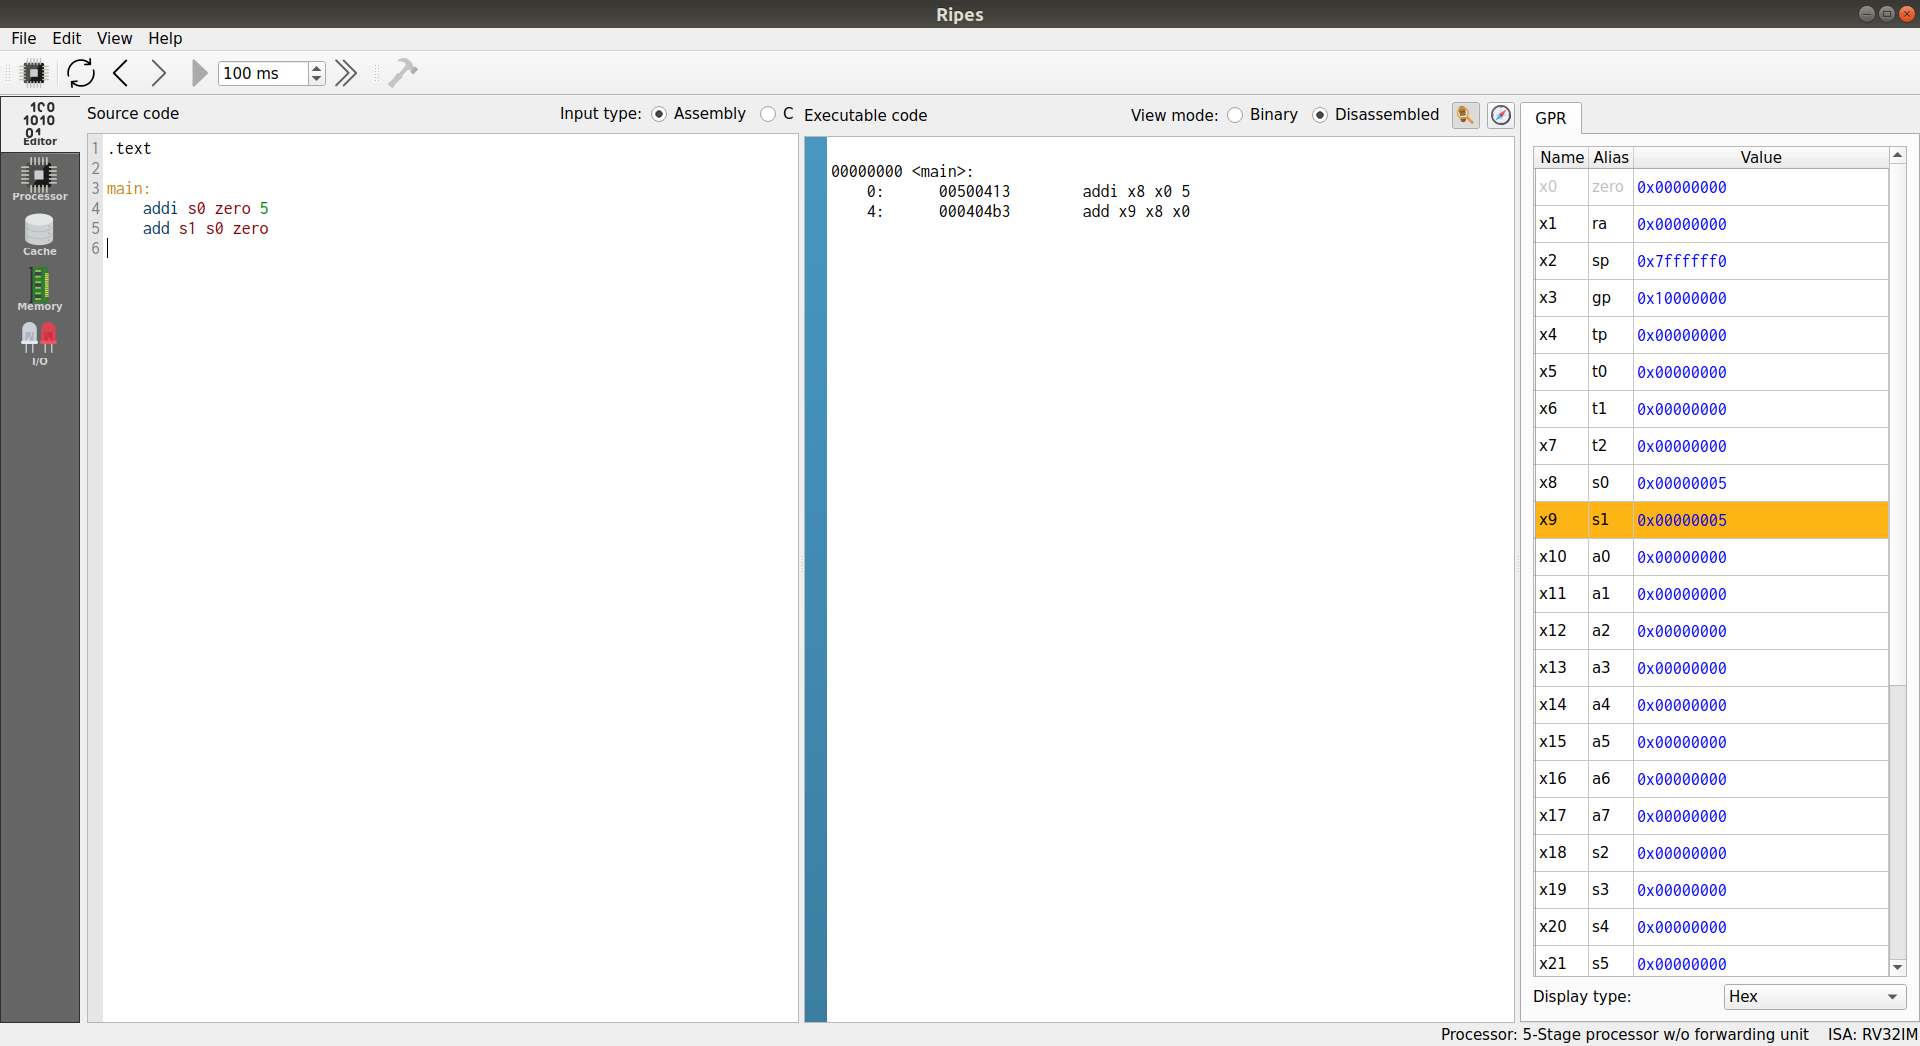
\includegraphics[scale=0.25]{Q1/hnf_end_editor.png}
  \caption{With hazard detection; Without forwarding;}
\end{figure}


\newpage
\section{5 Stage, without forwarding, with hazard detection}

\subsection{}
\subsubsection*{Code}
\begin{verbatim}
.text

main:
    addi s0 zero 5
    add s1 s0 zero
\end{verbatim}

\subsubsection*{Behaviour}
At the end of the program, we expect registers \verb!s0! and \verb!s1! to have value 5. \\
Without forwarding, we observe that ID for second instruction takes 3 cycles (2 stalls). \\
There are no stalls with forwarding.

\subsubsection*{Screenshots}
\begin{figure}[H]
  \centering
  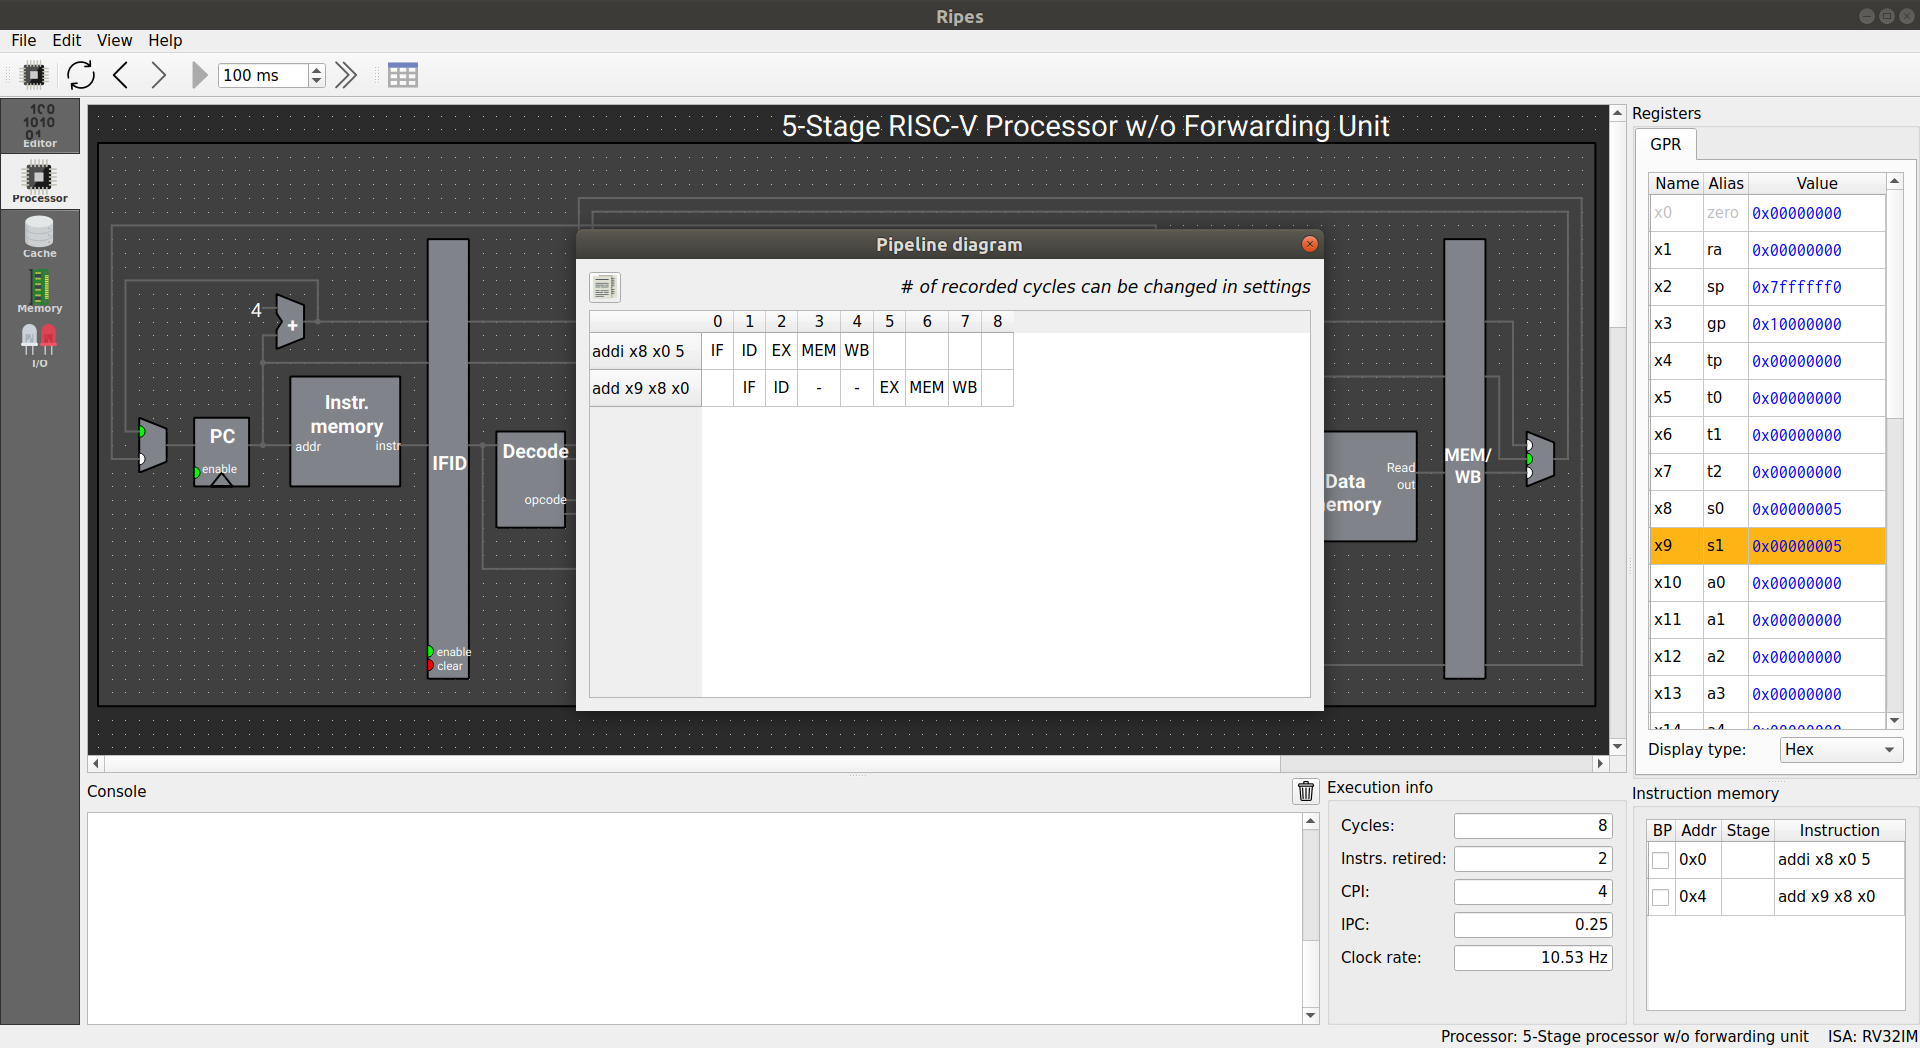
\includegraphics[scale=0.25]{Q2/a_hnf_end_pipeline.png}
  \caption{With hazard detection; Without forwarding;}
\end{figure}
\begin{figure}[H]
  \centering
  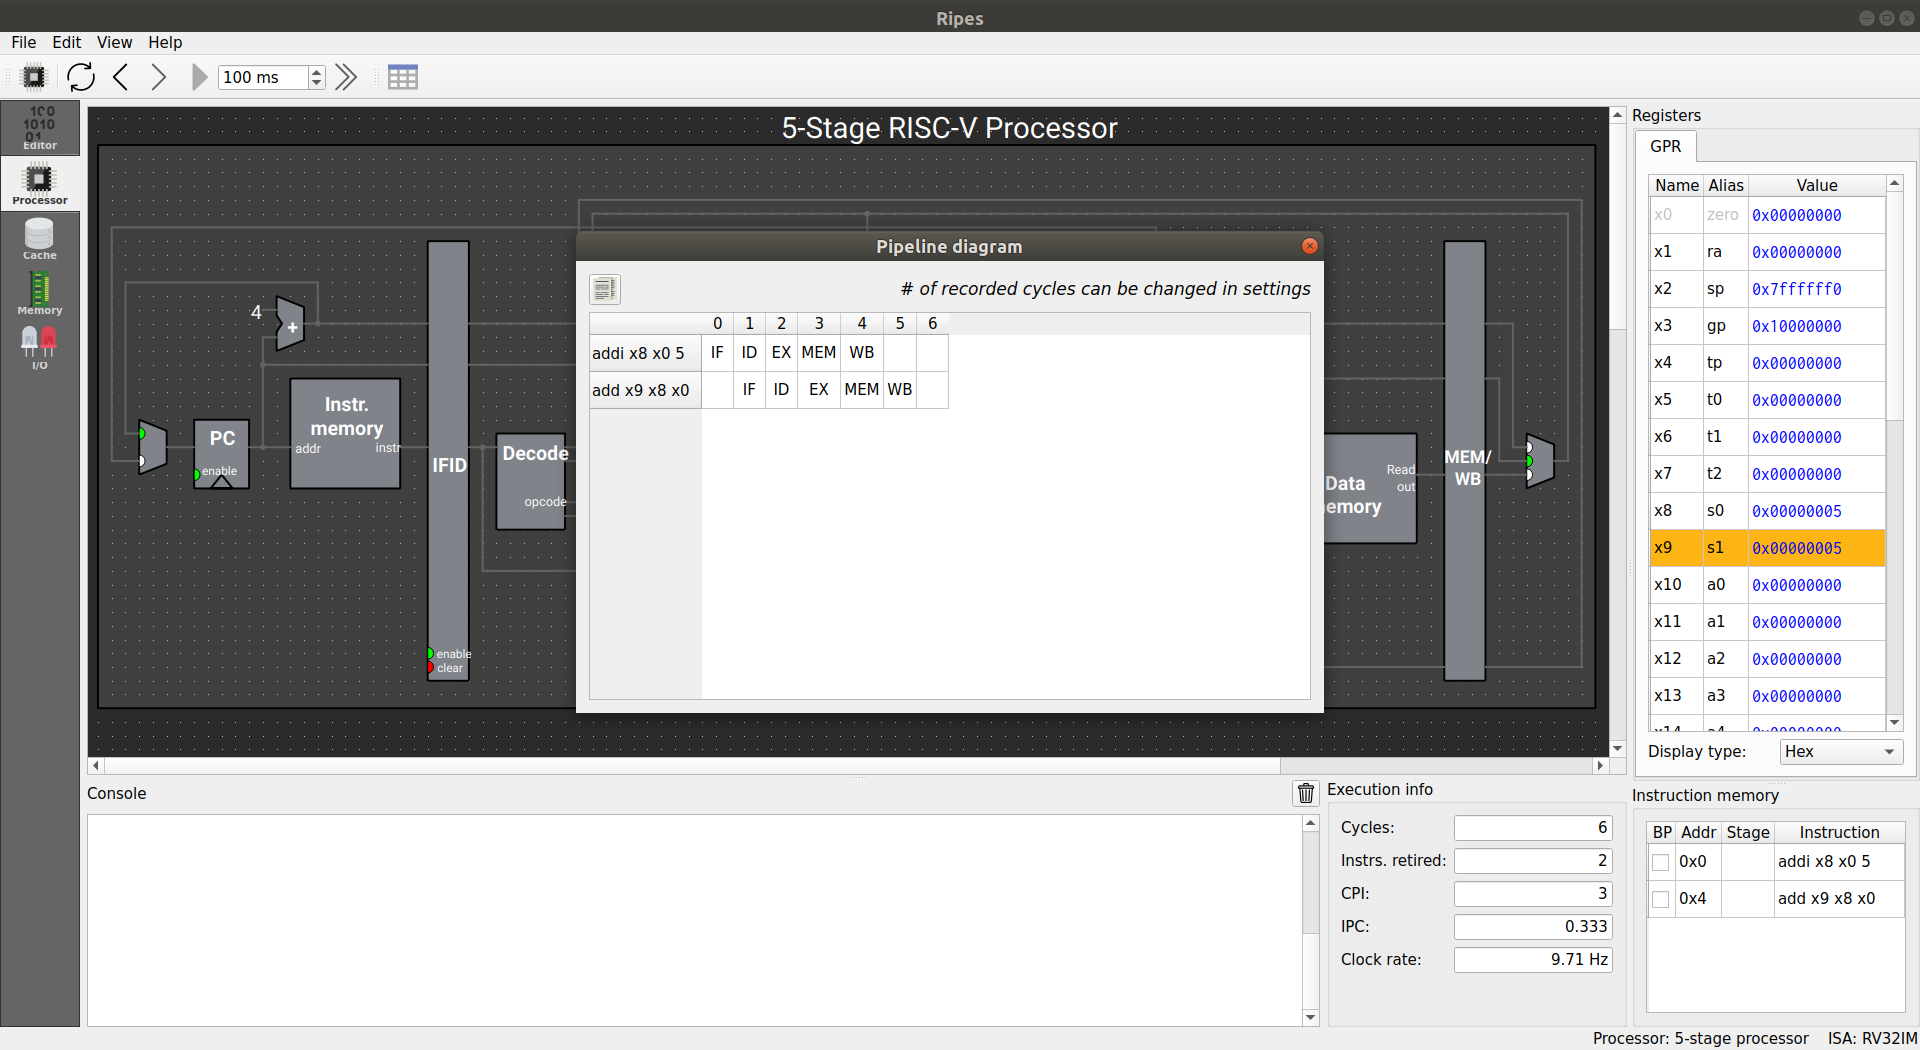
\includegraphics[scale=0.25]{Q2/a_hf_end_pipeline.png}
  \caption{With hazard detection; With forwarding;}
\end{figure}

\subsection{}
\subsubsection*{Initial Code}
\begin{verbatim}
.text

main:
    addi s0 zero 5
    add s1 s0 zero
    addi s2 zero 6
    addi s3 zero 7
\end{verbatim}

\subsubsection*{Optimized Code}
\begin{verbatim}
.text

main:
    addi s0 zero 5
    addi s2 zero 6
    addi s3 zero 7
    add s1 s0 zero
\end{verbatim}

\subsubsection*{Behaviour}
At the end of both the program, we expect registers \verb!s0! and \verb!s1! to have value 5, register \verb!s2! to have value 6 and, register \verb!s3! to have value 7.

\subsubsection*{Screenshots}
\begin{figure}[H]
  \centering
  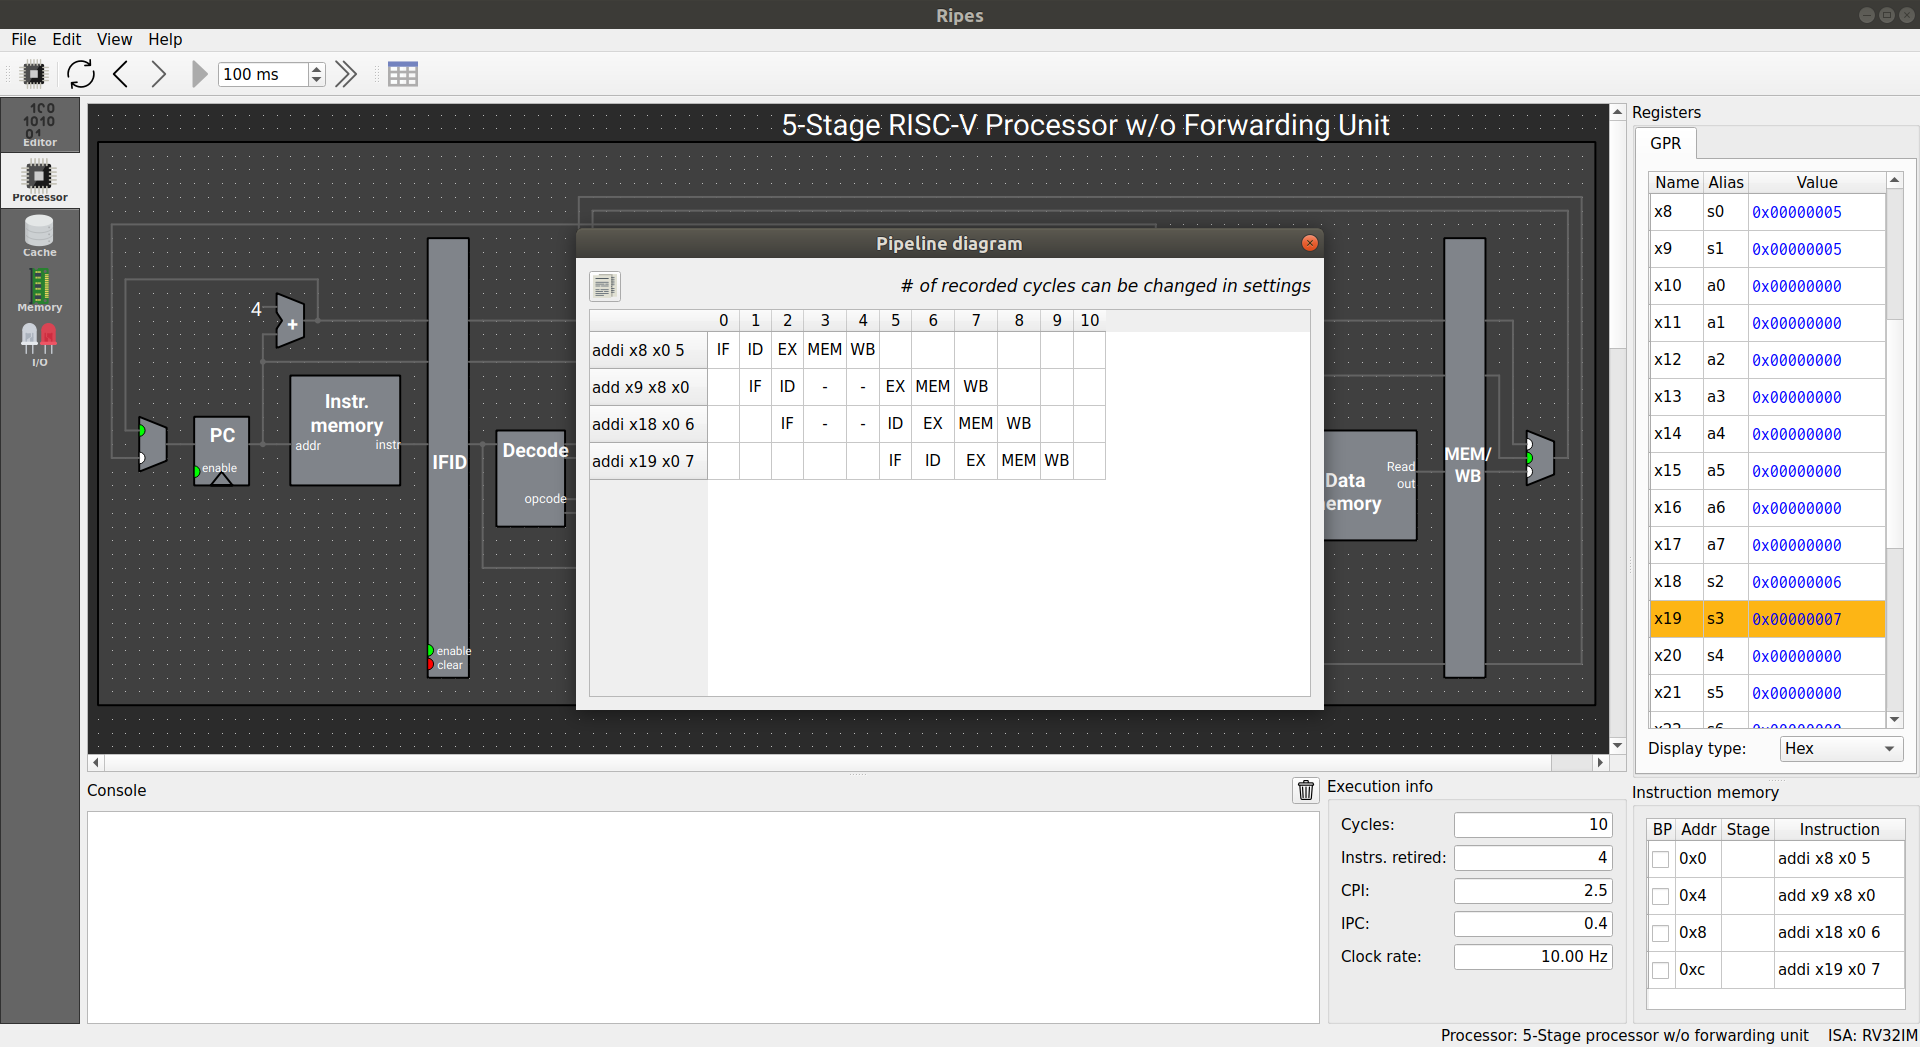
\includegraphics[scale=0.25]{Q2/b_init_hnf_end_pipeline.png}
  \caption{With hazard detection; Without forwarding; Initial code}
\end{figure}
\begin{figure}[H]
  \centering
  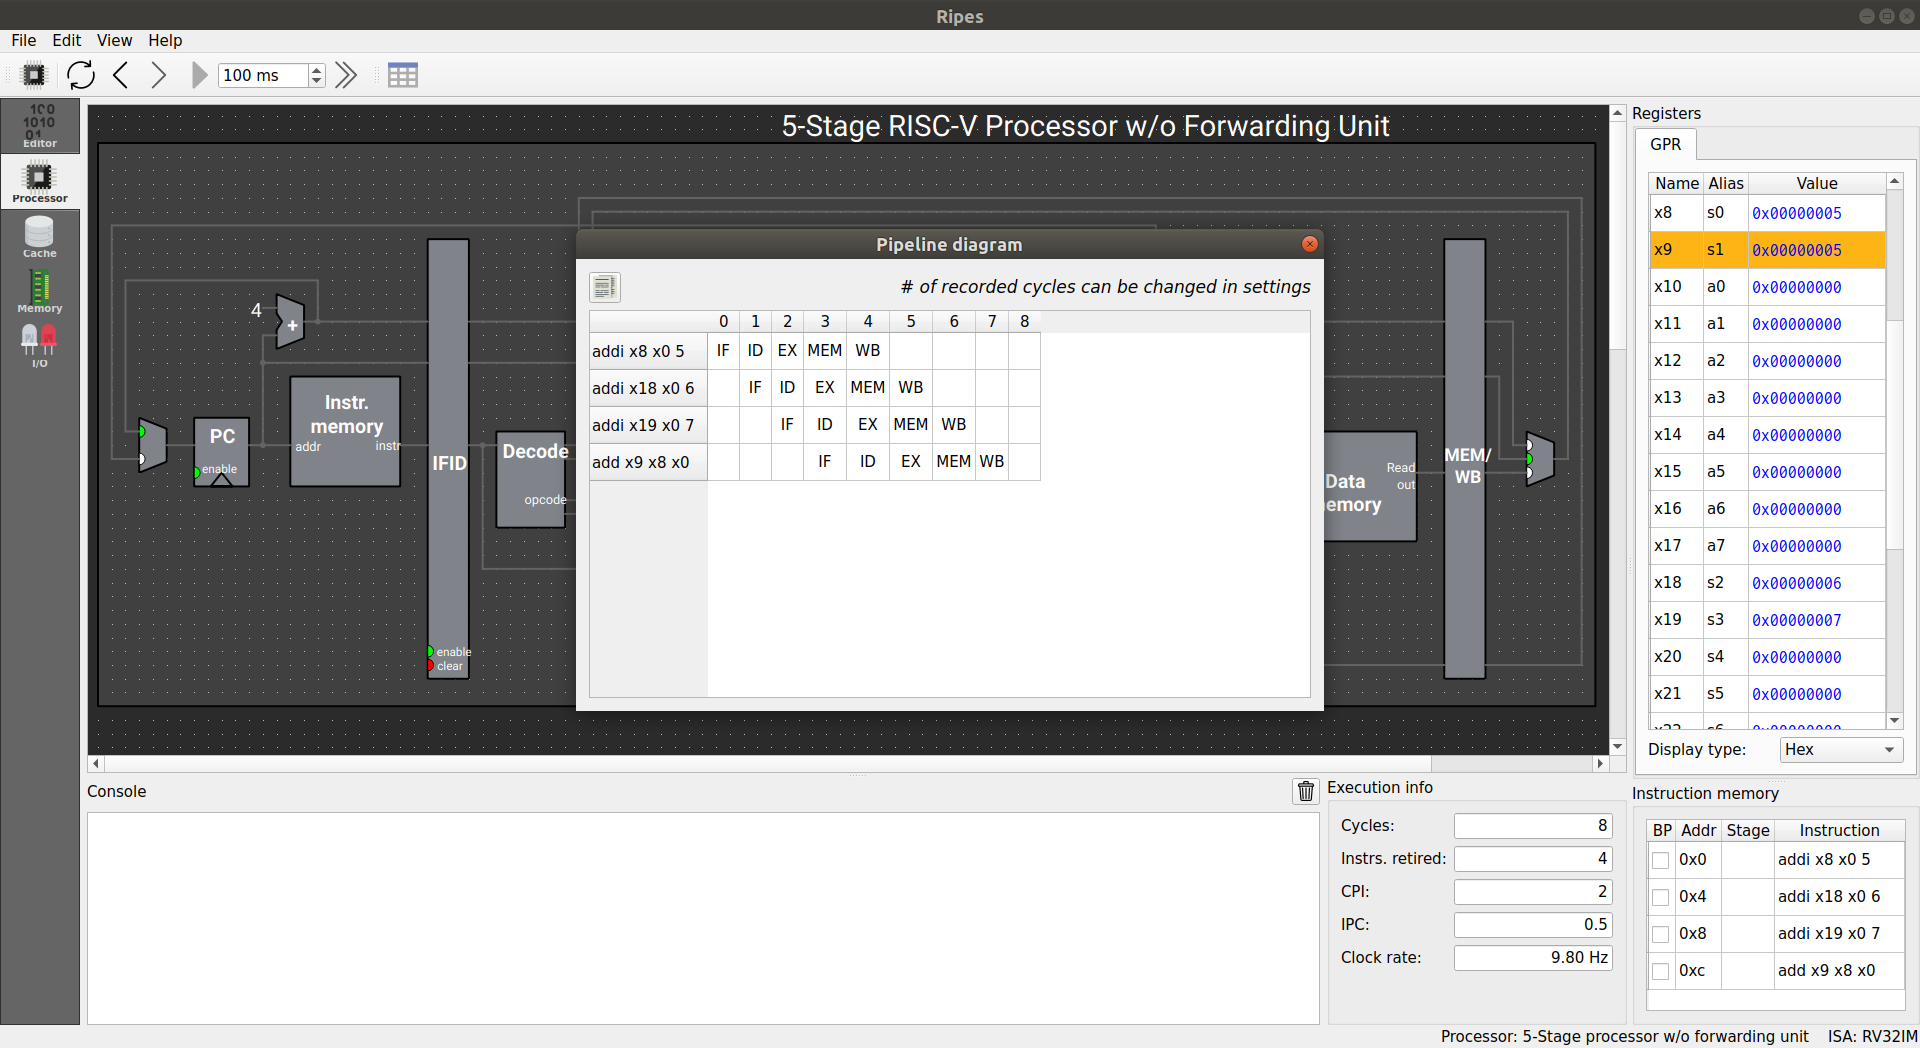
\includegraphics[scale=0.25]{Q2/b_opt_hnf_end_pipeline.png}
  \caption{With hazard detection; With forwarding; Optimized code}
\end{figure}


\newpage
\section{Stalls and Forwarding}

\subsection{}
Address input of data memory and EX/MEM pipeline after 4th cycle is \verb!0x0000000a!.
\begin{figure}[H]
  \centering
  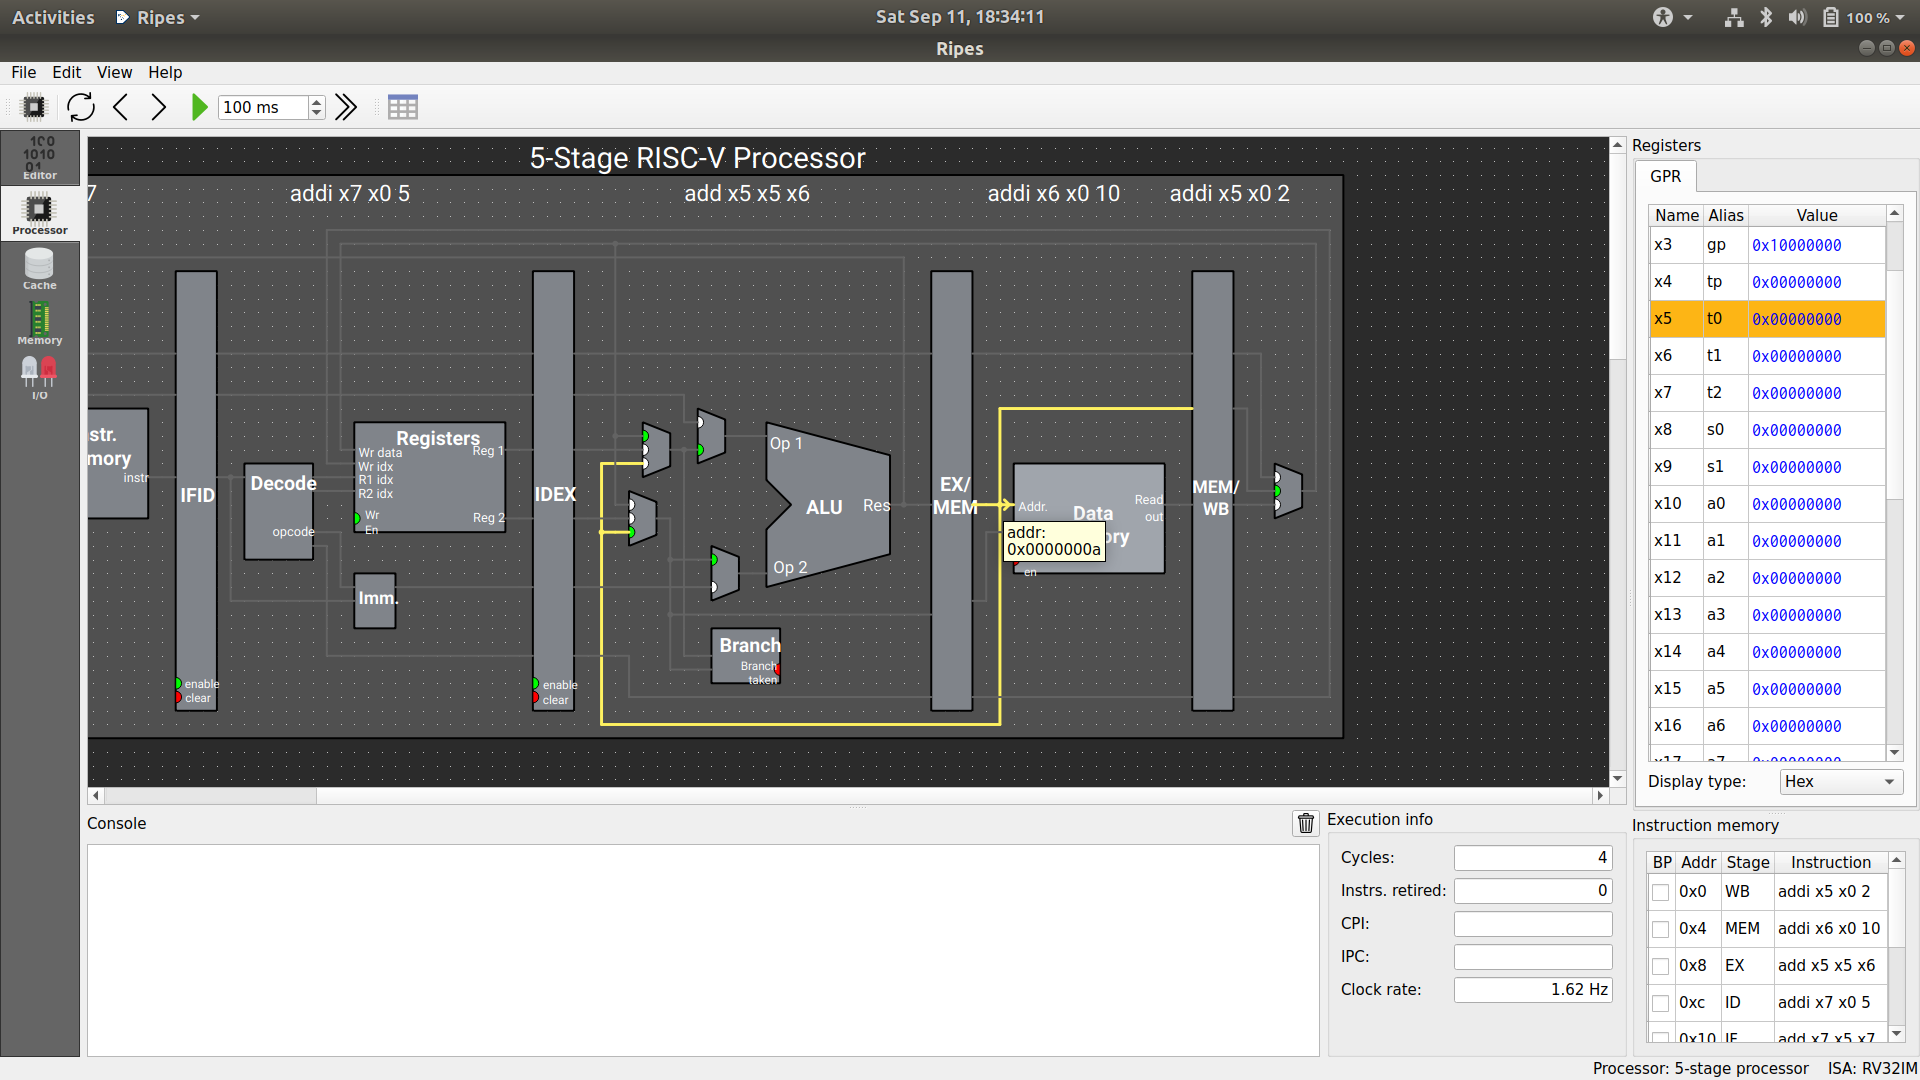
\includegraphics[scale=0.22]{Q3/hf_datapath.png}
  \caption{With hazard detection; With forwarding;}
\end{figure}

\subsection{}
R2 idx input of registers block and decoder after 10th cycle is \verb!0x01!.
\begin{figure}[H]
  \centering
  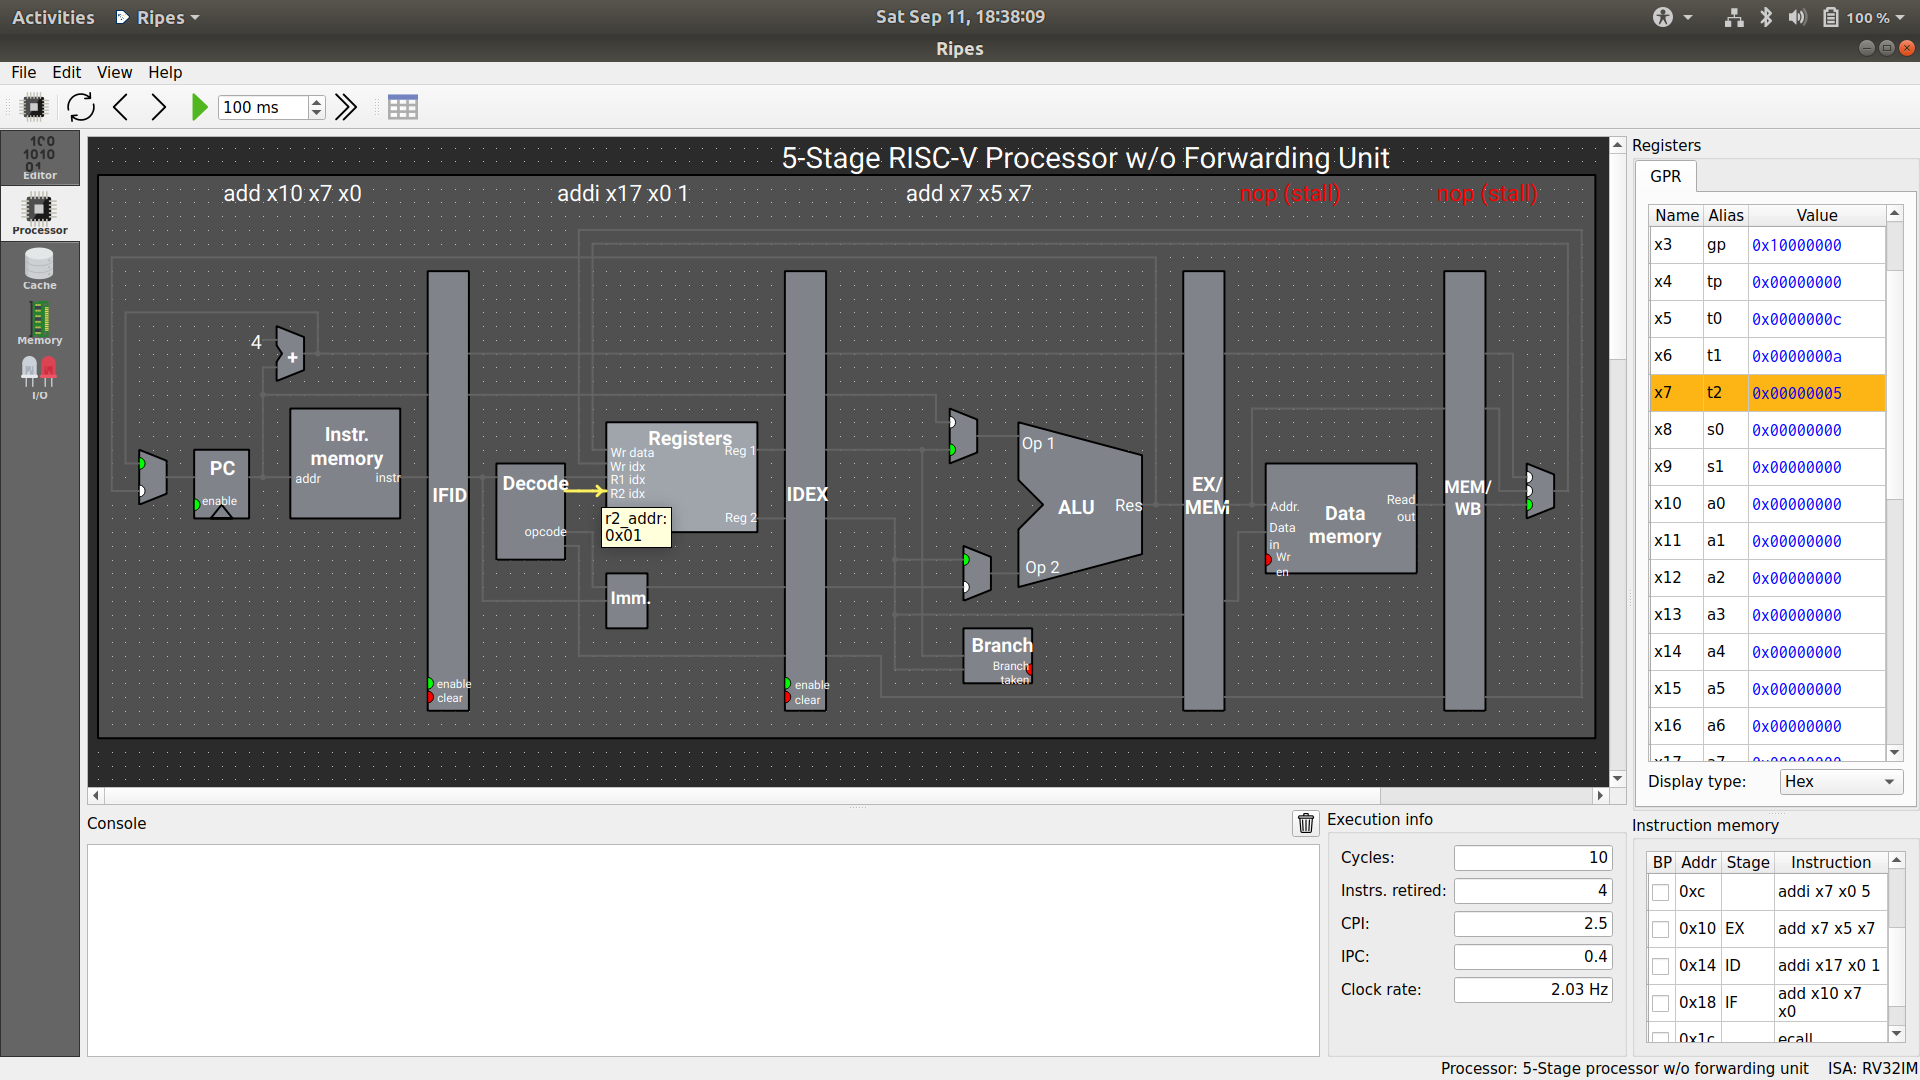
\includegraphics[scale=0.22]{Q3/hnf_datapath.png}
  \caption{With hazard detection; Without forwarding;}
\end{figure}

\subsection{}
The value stored in \verb!opcode_exec_out! datapath after 4 cycles is \verb!0x13!.
\begin{figure}[H]
  \centering
  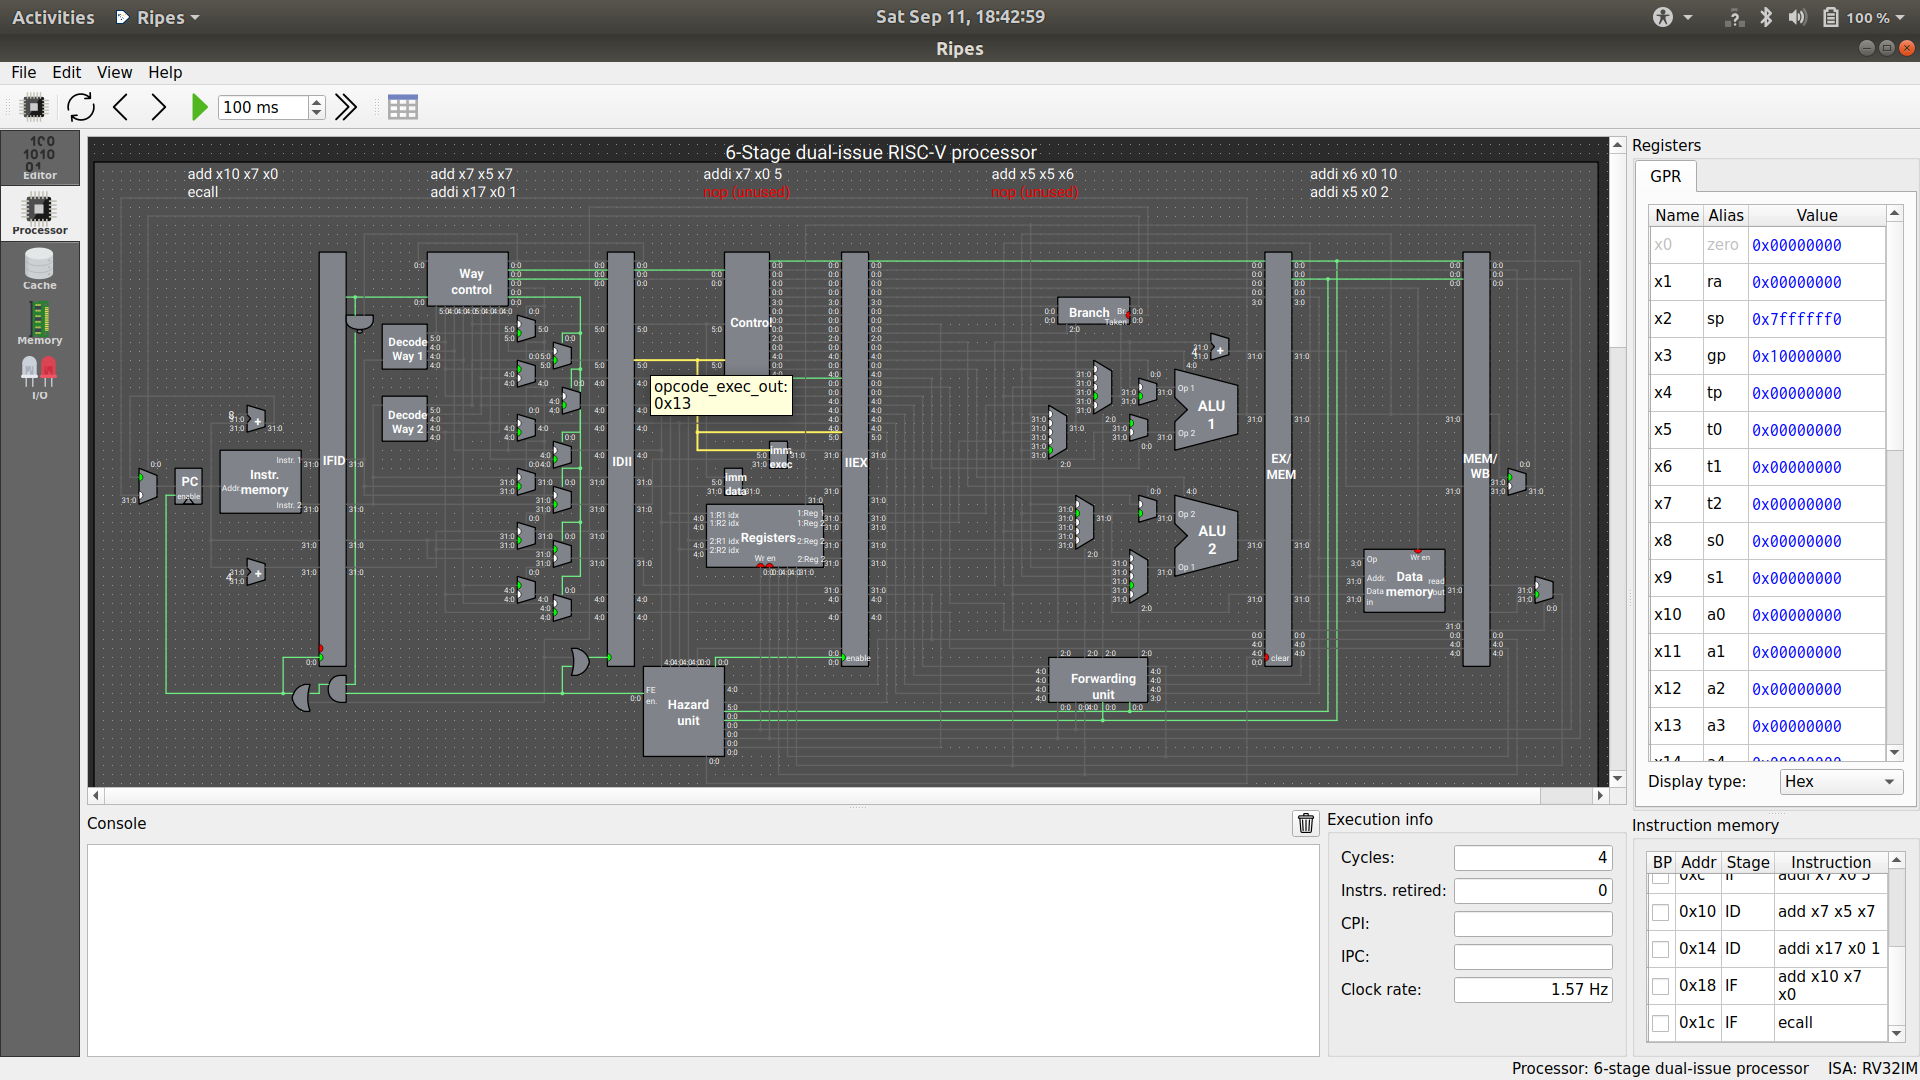
\includegraphics[scale=0.22]{Q3/6di_datapath.png}
  \caption{6-stage dual-issue processor}
\end{figure}

\subsection{}
\begin{figure}[H]
  \centering
  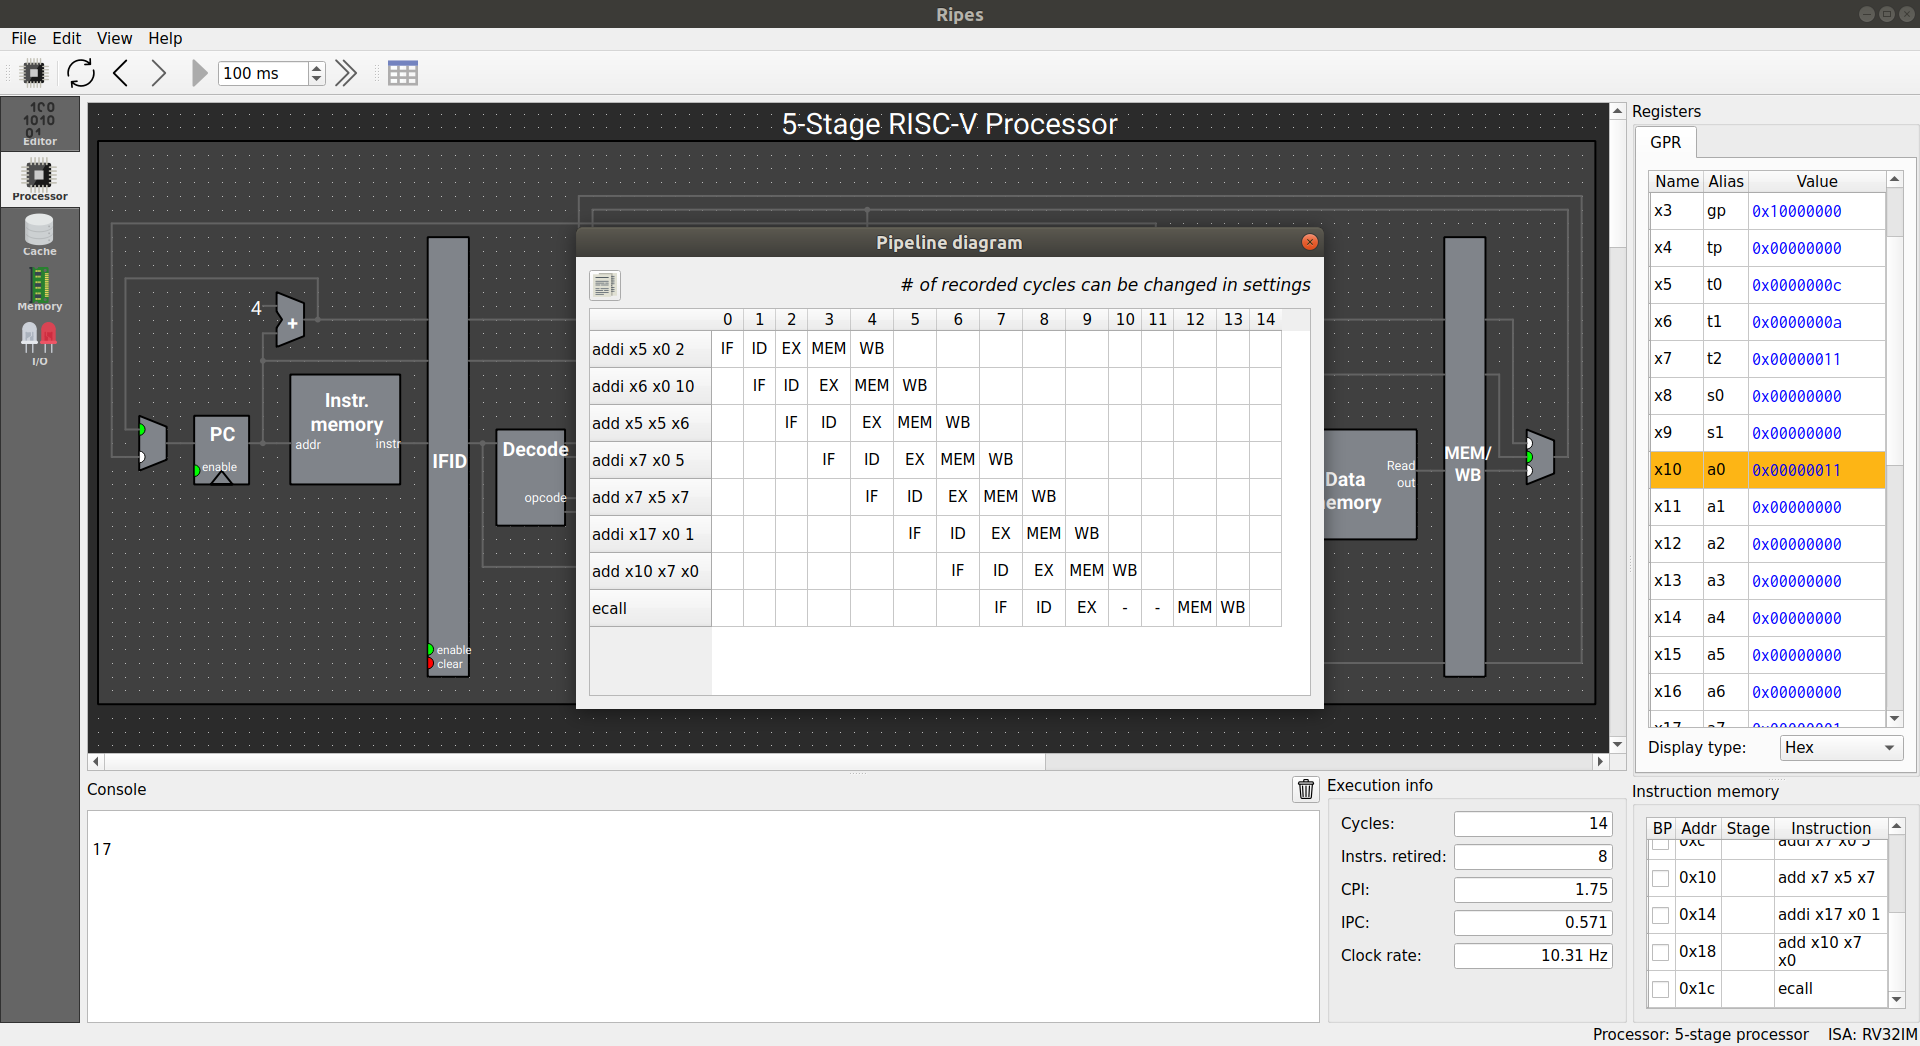
\includegraphics[scale=0.22]{Q3/hf_pipeline.png}
  \caption{With hazard detection; With forwarding; \textbf{Takes 14 cycles}}
\end{figure}
\begin{figure}[H]
  \centering
  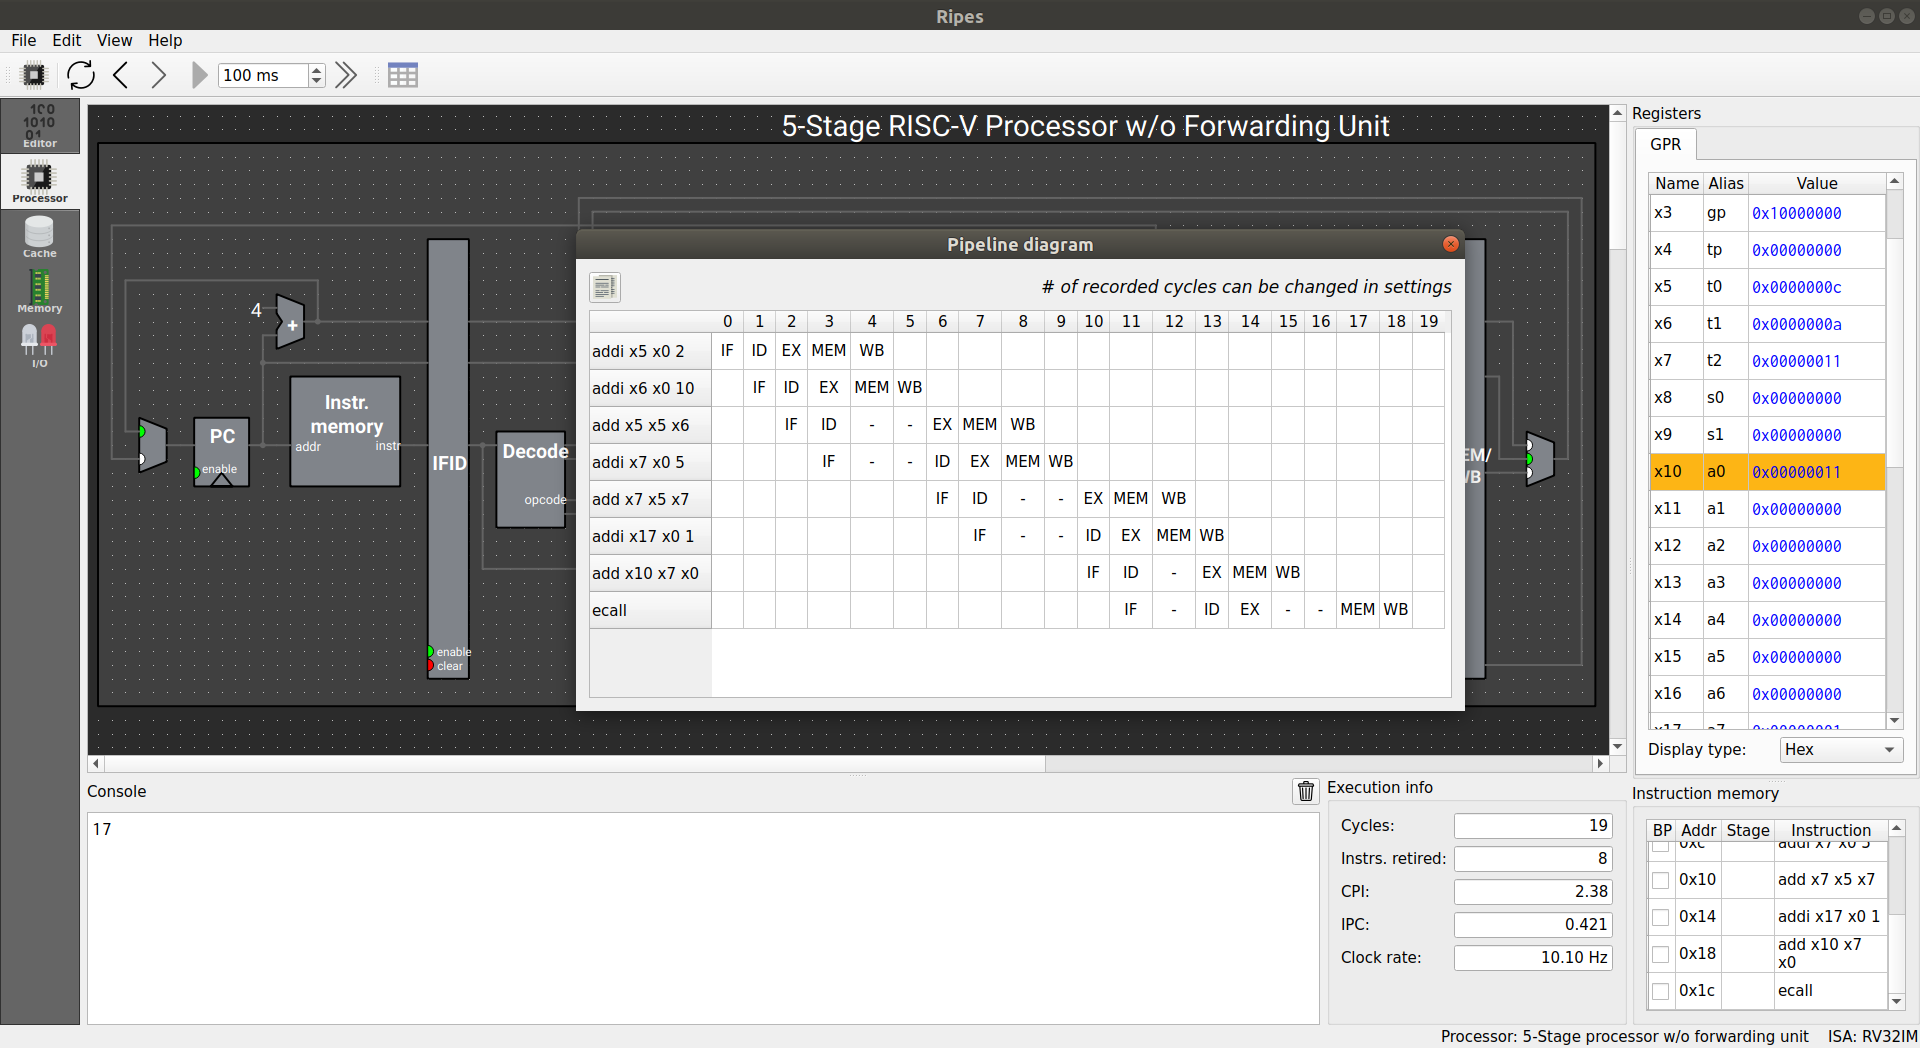
\includegraphics[scale=0.22]{Q3/hnf_pipeline.png}
  \caption{With hazard detection; Without forwarding; \textbf{Takes 19 cycles}}
\end{figure}
\begin{figure}[H]
  \centering
  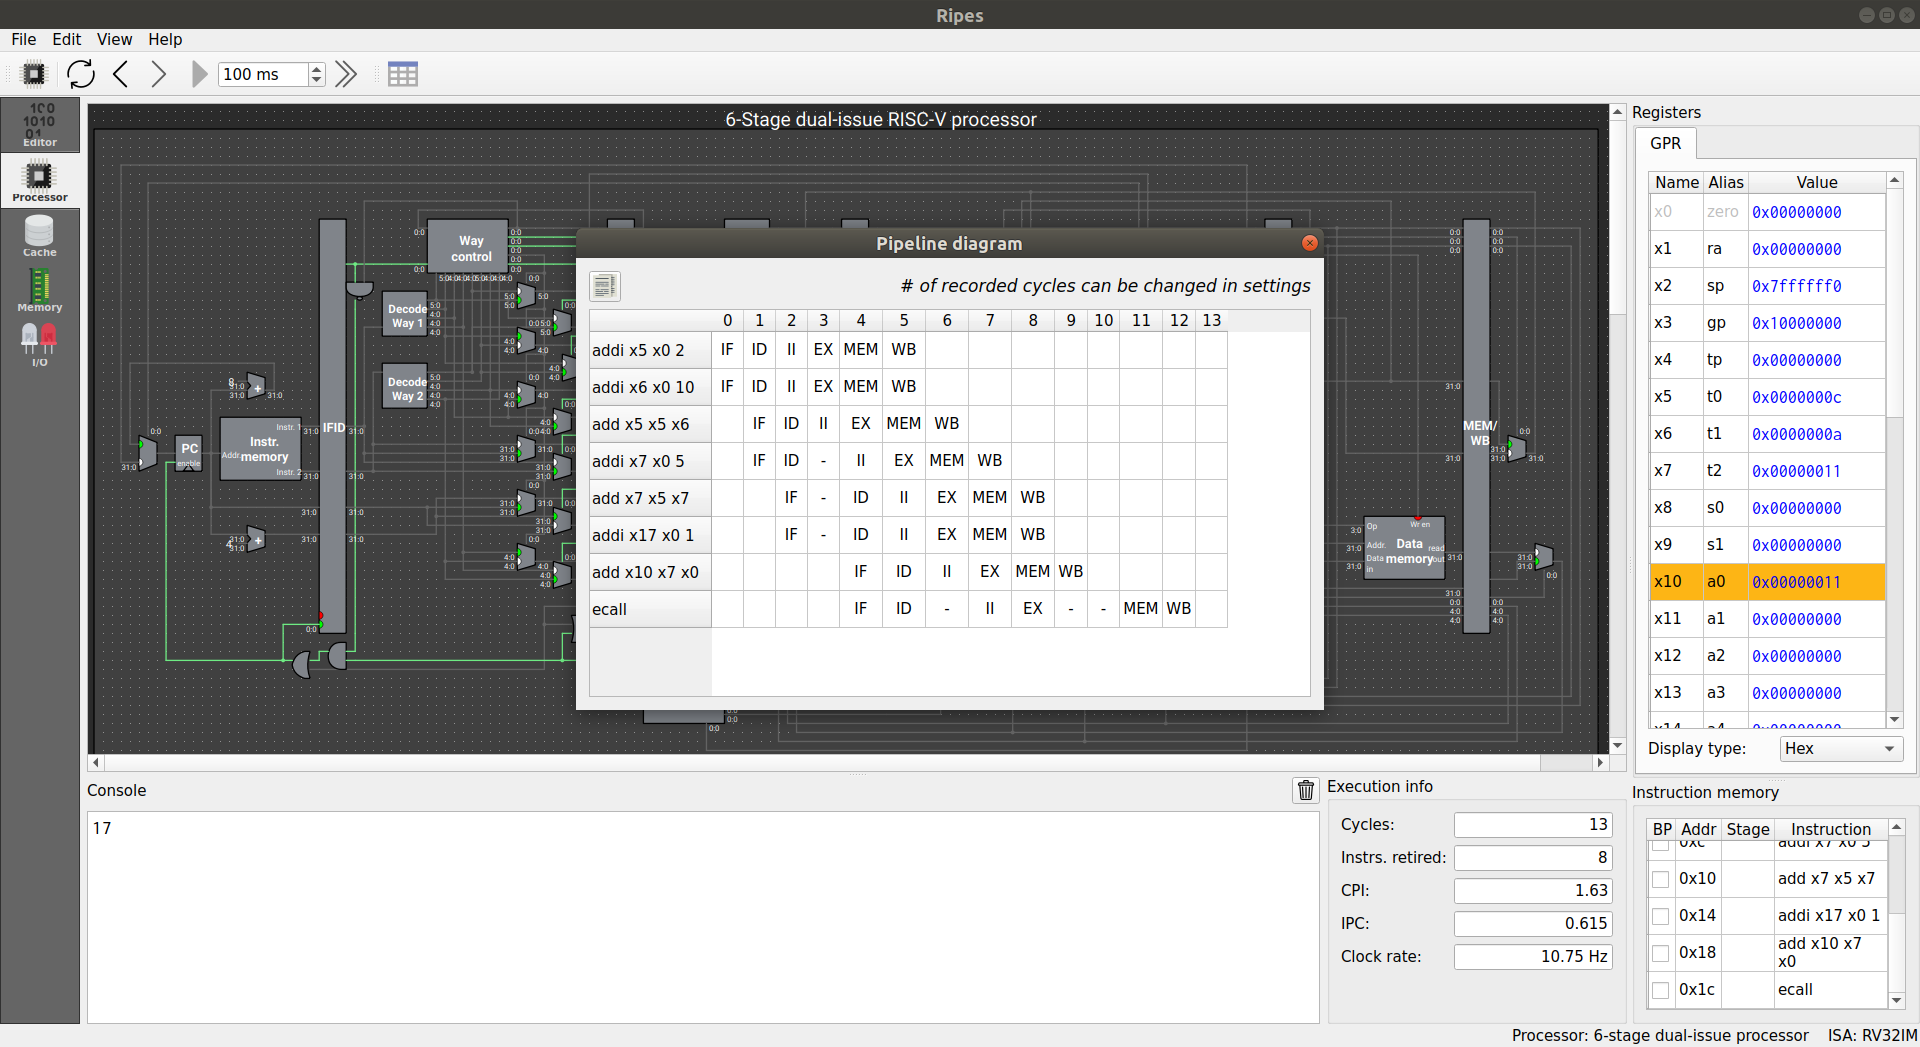
\includegraphics[scale=0.22]{Q3/6di_pipeline.png}
  \caption{6-stage dual-issue processor; \textbf{Takes 13 cycles}}
\end{figure}

\subsection{}
The major issue is that the value of register \verb!a7! is not updated before \verb!ecall! reaches ID stage. There is no system call with \verb!a7! as 0, so an error occurs. \\
\begin{figure}[H]
  \centering
  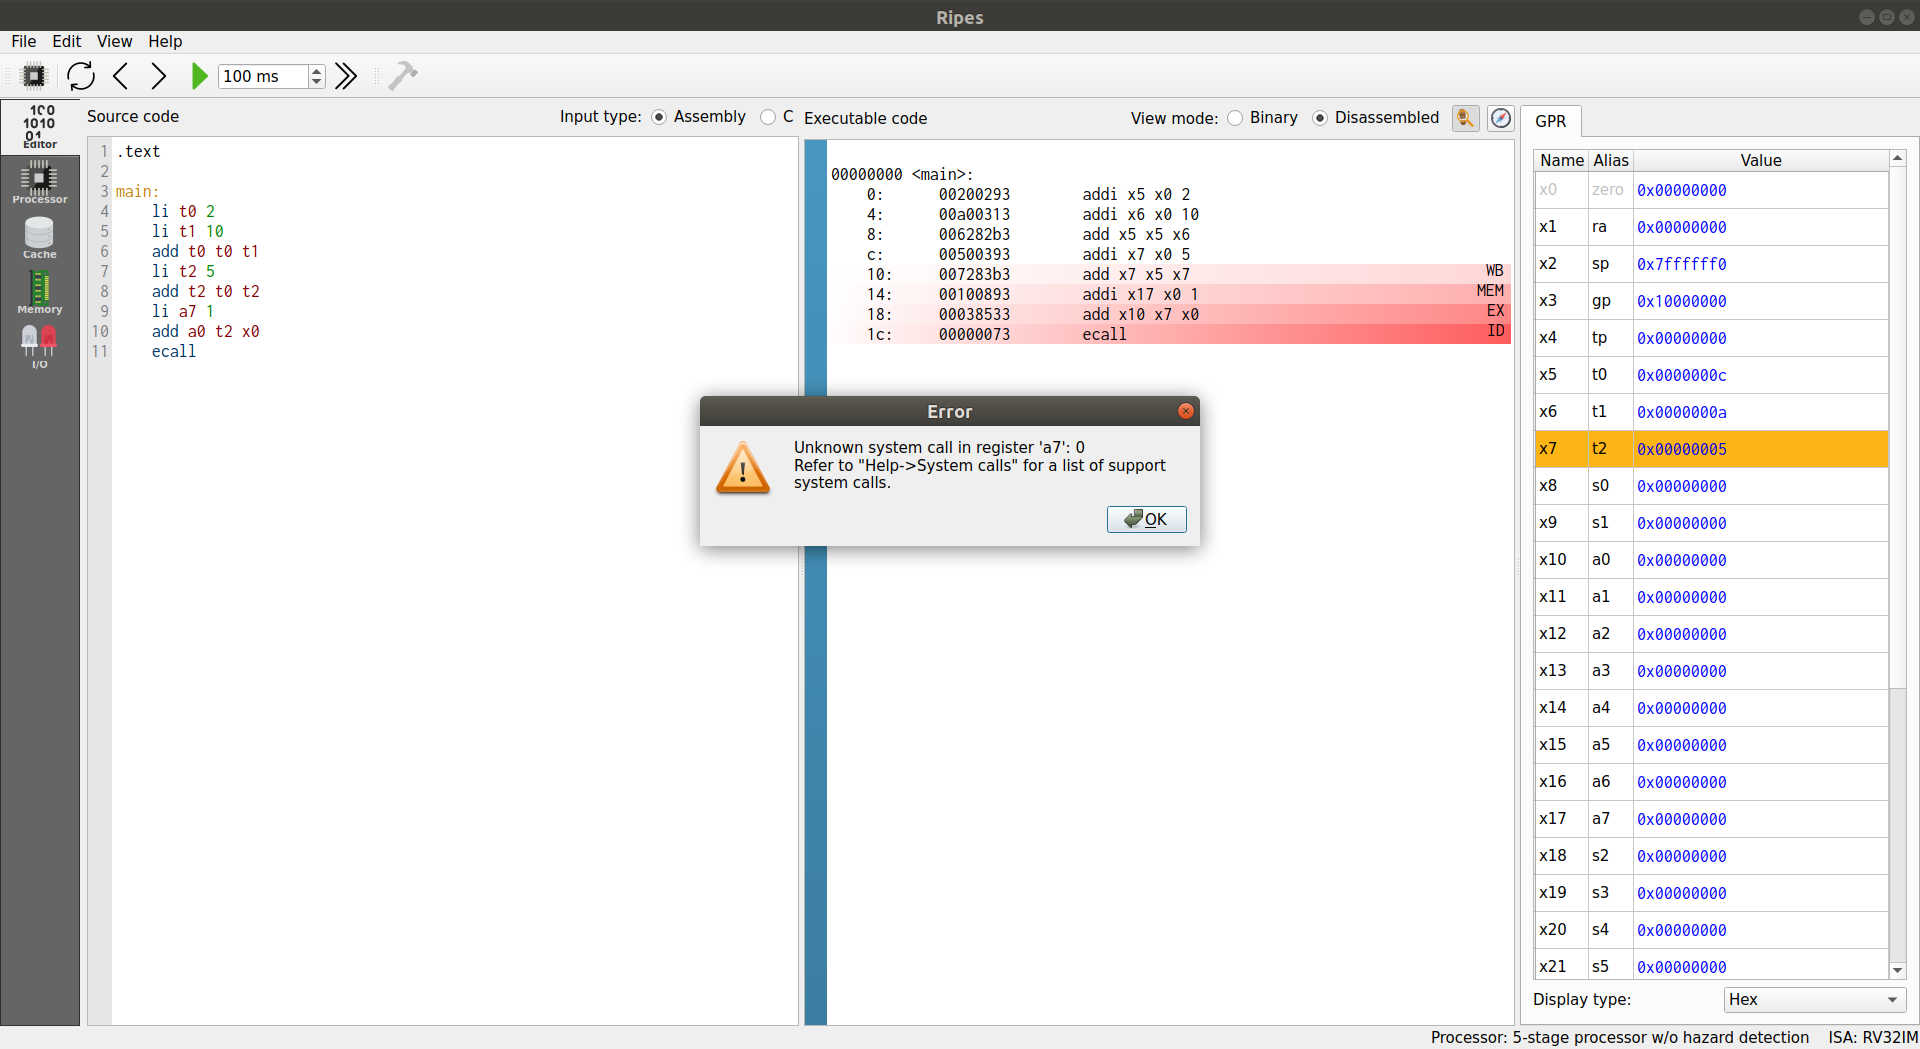
\includegraphics[scale=0.22]{Q3/nhf_error_init.png}
  \caption{Without hazard detection; With forwarding; Error}
\end{figure}

One simple solution is to add \verb!nop!s before \verb!ecall!. \\
If we add two \verb!nop!s, the error goes away but we end up with output 0 instead of 17. \\
This happens because the value of register \verb!a0! is not updated before \verb!ecall! sends to signal to the console. \\
If we add one more \verb!nop!, the output is 17. \\

Updated code:
\begin{verbatim}
.text

main:
    li t0 2
    li t1 10
    add t0 t0 t1
    li t2 5
    add t2 t0 t2
    li a7 1
    add a0 t2 x0
    nop
    nop
    nop
    ecall
\end{verbatim}

\begin{figure}[H]
  \centering
  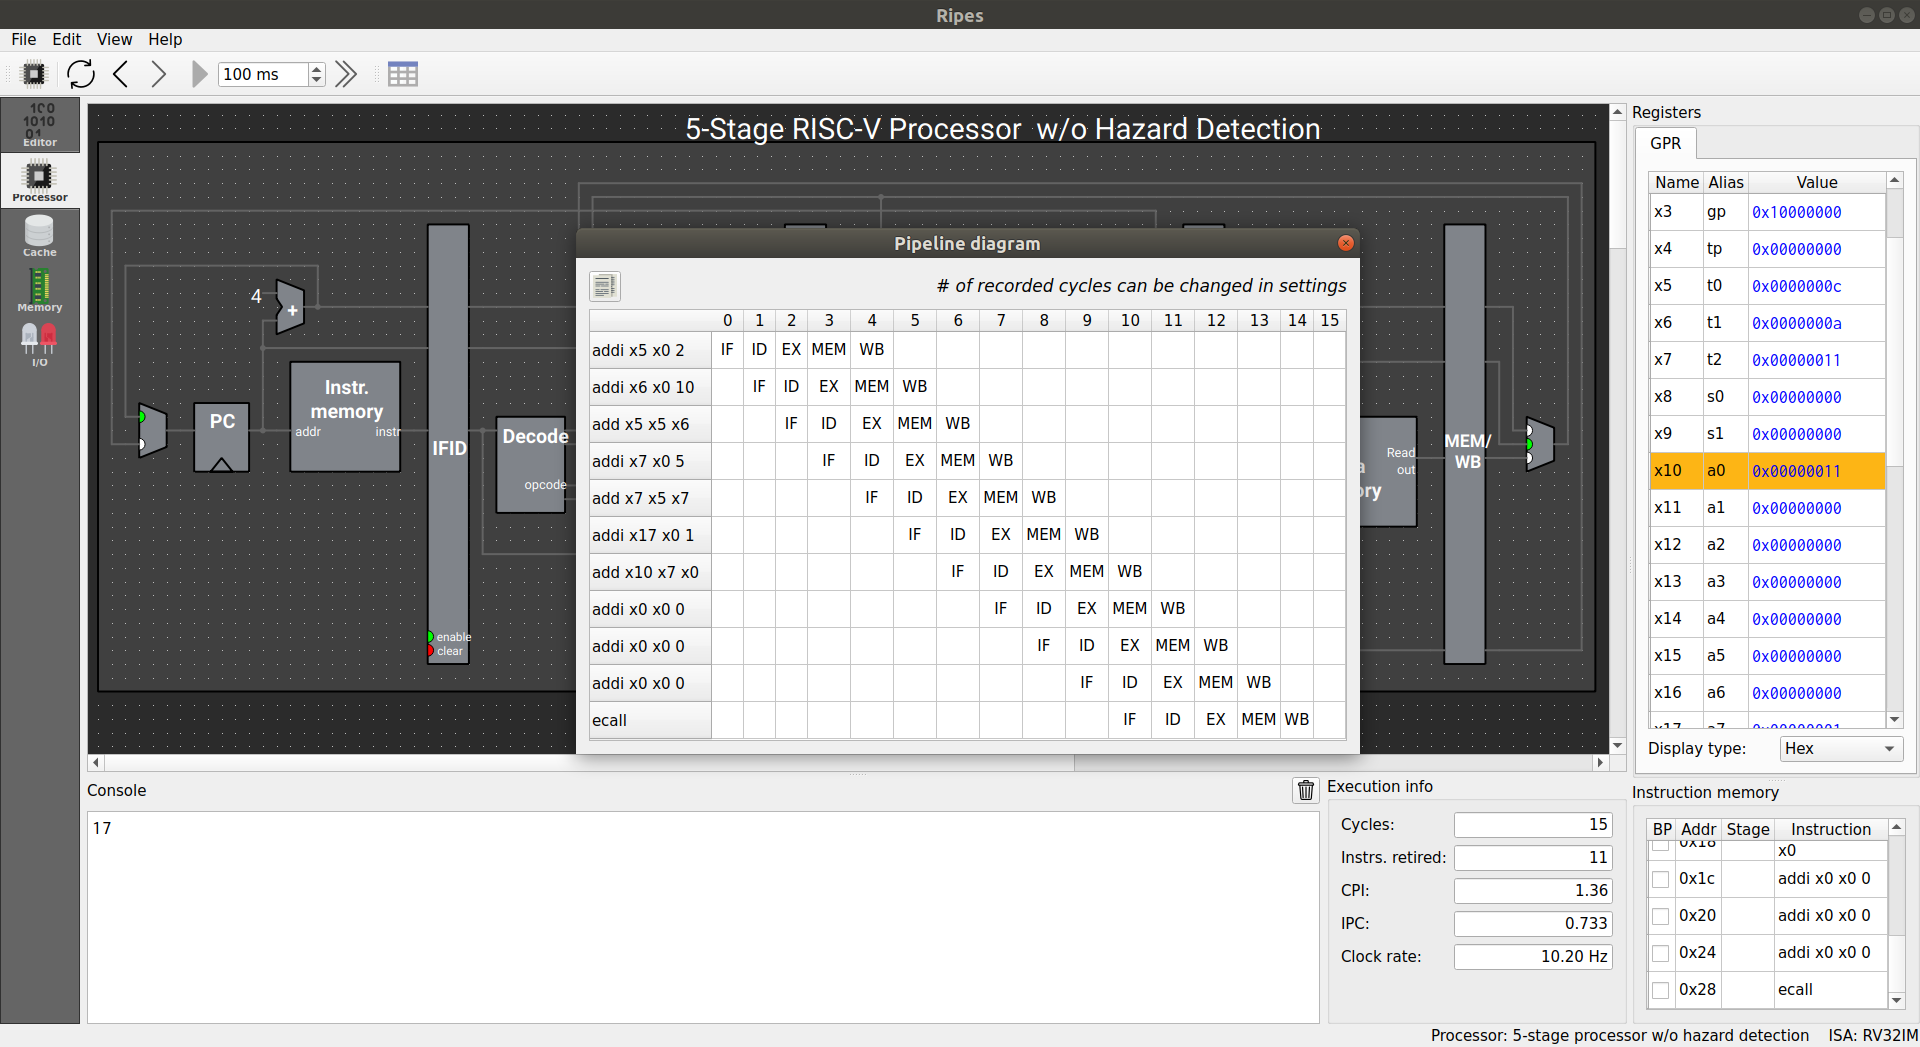
\includegraphics[scale=0.22]{Q3/nhf_console_fixed.png}
  \caption{Without hazard detection; With forwarding; Fixed bug; \textbf{Takes 15 cycles}}
\end{figure}

\newpage
\section{Maximising Efficiency}

\subsubsection*{Code}
\begin{verbatim}
.text

main:
    li a0 1
    li a7 1
    li a1 2
    li a6 3
    add a0 a0 a7
    li a7 5
    add a1 a1 a6
    li a6 8
    add a0 a0 a7
    li a7 13
    add a1 a1 a6
    li a6 21
    add a0 a0 a7
    li a7 34
    add a1 a1 a6
    li a6 55
    add a0 a0 a7
    li a7 1
    add a1 a1 a6
    add a0 a0 a1
    ecall
\end{verbatim}

\subsubsection*{Behaviour}
Output is $1+1+2+3+5+8+13+21+34+55 = 134$. \\
Minimum of 29 cycles are required. \\
Minimum of 4 registers are required to finish in 29 cycles.

\subsubsection*{Explanation for minimum cycles}
We require 10 \verb!li! instructions and at least 9 \verb!add! instructions (to add 10 integers). \\
Then there are two more instructions - one \verb!li! instruction to set \verb!a7! register to 1 and one \verb!ecall! instruction to output on console. \\
Without stalls, it would take minimum of 25 cycles (21 + 4). \\

Read of a particular register requires 2 instructions after previous write operation to the register in order to avoid stalls. \\

We can have one temporary variable storing the sum. \\
This would require updating the variable only after reading two integers, which would cause consecutive additions once we have read all integers. ($\sim 10$ stalls for this). \\

Instead we can use two temporary variables for storing partial sum and then add them at the end to obtain the sum. \\
This way we can update the variables alternatively after reading an integer. \\
This would cause two stalls at the end when we would have to add the two variables just after updating one of the variables. \\

For more than two temporary variables, the number of stalls at the end to obtain the sum would only increase. \\

In addition to this, we would have another two stalls during \verb!ecall! instruction. \\
This for some reason seems to be inevitable even after including \verb!nop!s.

\subsubsection*{Explanation for minimum registers}
We read 4 integers before first sum as we would be adding first two integers and we need a gap of two instructions before we can add without stall. \\
During the flow, we require 2 registers to store partial sum and 2 registers to store integer input. \\
For the syscall, we would require \verb!a0! and \verb!a7! registers. \\
With proper arrangement we can satisfy our need with only 4 registers without adding anymore stalls. \\
\verb!a0! and \verb!a1! store partial sum. \\
\verb!a7! and \verb!a6! store integer input. \\

\begin{figure}[H]
  \centering
  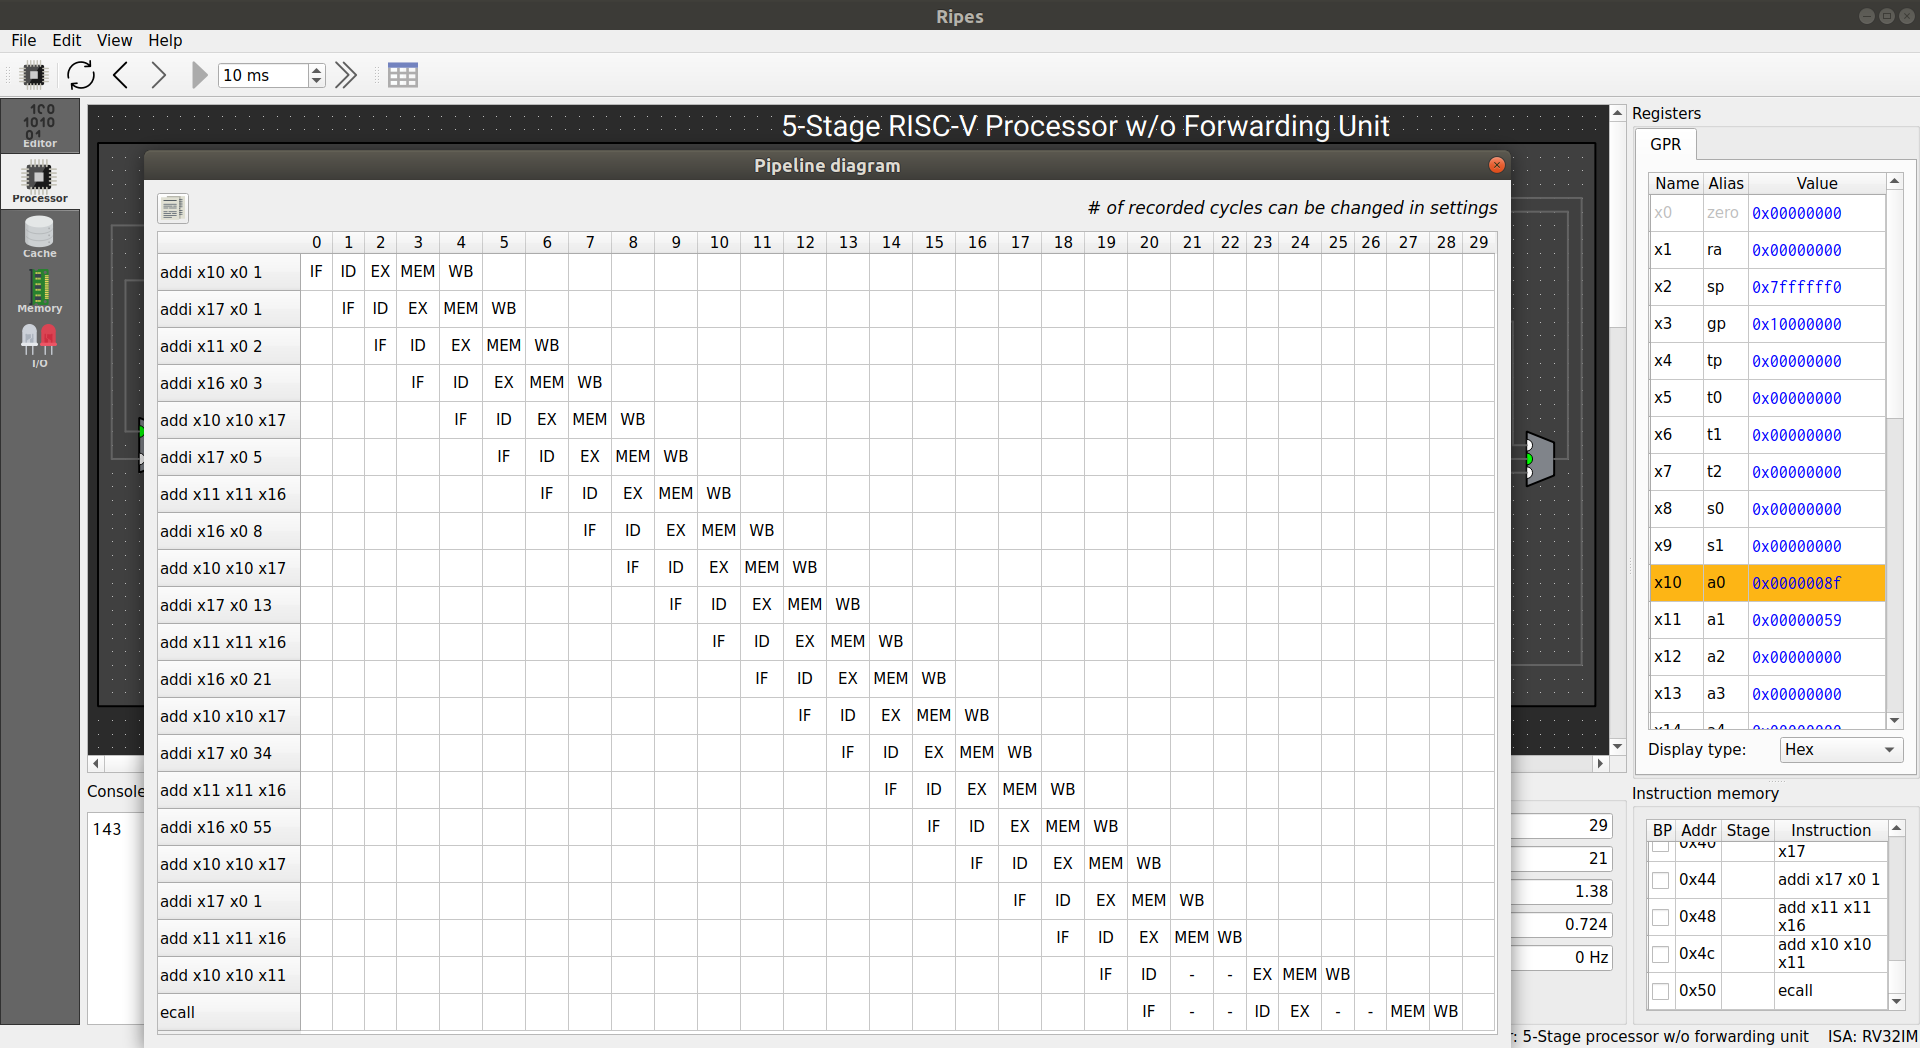
\includegraphics[scale=0.22]{Q4/hnf_pipeline.png}
  \caption{With hazard detection; Without forwarding; \textbf{Requires 29 cycles and 4 registers}}
\end{figure}

\end{document}
